% FILE: figures/k0_to_k1_transition.tex
% Transition from K0 to K1

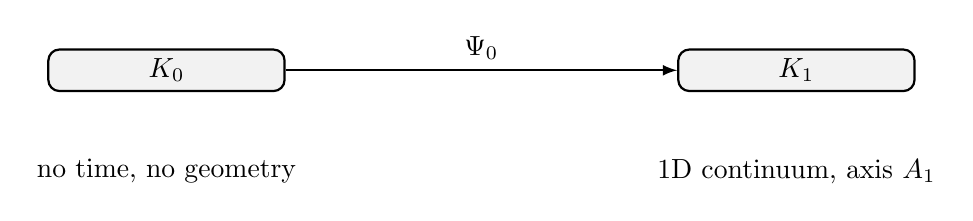
\begin{tikzpicture}[>=latex,thick]
  % K0
  \node[draw, rounded corners, fill=gray!10, minimum width=3cm] (K0) at (-4,0) {$K_0$};
  \node[anchor=north] at (-4,-1.0) {no time, no geometry};

  % K1
  \node[draw, rounded corners, fill=gray!10, minimum width=3cm] (K1) at (4,0) {$K_1$};
  \node[anchor=north] at (4,-1.0) {1D continuum, axis $A_1$};

  % Arrow with label
  \draw[->] (K0) -- node[above] {$\Psi_0$} (K1);
\end{tikzpicture}
